\pagestyle{myheadings}
\markboth{Quasar Redshift}{Quasar Redshift}
\setcounter{page}{1}

\begin{center}
{\Huge\bf Quasar Redshift}
\end{center}

\vspace{0.3cm}

{\large {\bf 1. Introduction}}

The aim of this Astronomical Exercise is to lead you through the process
of reduction, calibration and analysis of a real optical spectrum of a quasar 
in order that you can determine its redshift. Redshift is an important
quantity in astronomy because it allows us to determine the 
cosmological distance to an object, and therefore its luminosity.
While the redshift, $z$, of
the quasar is the ultimate objective of this process, along the way you
should gain a greatly improved understanding of the key reduction processes
of flat-fielding, sky subtraction, and wavelength calibration.

In your home directory there should be three two-dimensional spectra. 
These spectra are in files called
\begin{itemize}

\item{{\tt quasar.fits} - the spectrum of the target quasar.}

\item{{\tt flatfield.fits} - an exposure of the
inside of the dome illuminated by a tungsten lamp, which provides a
continuous spectrum of use for mapping the sensitivity variation of the
detector.} %({\em see Ap3 Observational Astronomy course notes}).

\item{{\tt arc.fits} - a spectrum of the Copper/Neon/Argon arc lamp (which
is located in the spectrograph). This provides emission lines at {\em
known} wavelength (see attached spectral atlas), thus enabling accurate
wavelength calibration of the target spectrum.}

\end{itemize}

{\large {\bf 2. Reduction Package}}

You are going to analyse the spectra using a set of software packages 
called {\sc iraf} (Image Reduction and Analysis
Facility\footnote{http://iraf.noao.edu/}). In your home directory you
will find a directory called {\tt iraf}. Change into this directory
(i.e. {\tt cd iraf}) and then type:

{\tt \verb,xgterm -sb &,}

\noindent
and from within the new terminal which appears, type:

{\tt cl}

\noindent
This will start {\sc iraf} which should then display a list of available
packages. The list of packages that these exercises will use are listed in the Appendix. These should be typed into the {\it login.cl} file so that you can access them without manually loading them in each time you access {\sc iraf} - the demonstrator should show you how to do this. To exit {\sc iraf} simply type {\tt logout}.

{\large {\bf 3. Displaying the spectra}}

The first thing to do is to display the three spectra, which is done
with the {\sc gaia} software package you used previously for the CCD
photometry exercise. From an xterm (not the {\sc iraf} window), type:

{\tt gaia quasar.fits \&}

which should display the two-dimensional quasar spectrum in a {\sc gaia}
window. When displayed by {\sc gaia} the two-dimensional
quasar spectrum should look something like Fig 3, with the quasar spectrum
itself appearing as a bright horizontal line superimposed on the night-sky
emission lines. The dispersion direction of the spectrum is
horizontal, with blue wavelengths to the left and red wavelengths to
the right.
\begin{figure}
\centerline{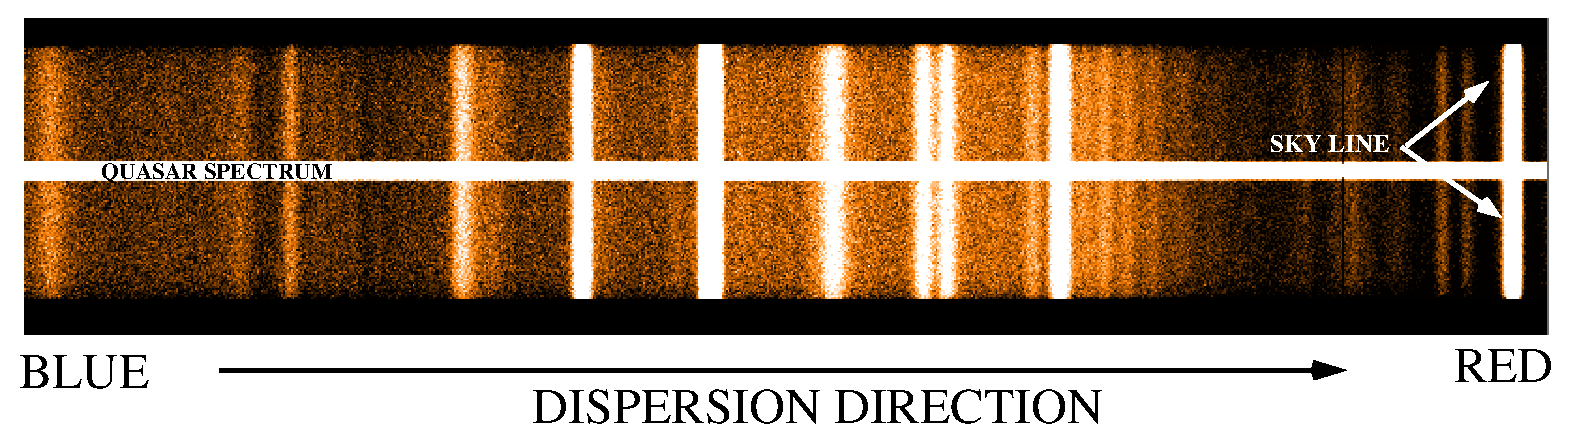
\psfig{file=spectrum_fig1.ps,width=16.0cm,angle=0}}
\caption{Two-dimensional quasar spectrum as displayed by {\sc gaia}}
\end{figure}

Display the other two spectra in new {\sc gaia} windows and familiarize yourself with them. The
arc spectrum should consist of a series of bright vertical emission
lines. These emission lines have known wavelengths, and will be used 
to wavelength calibrate the quasar spectrum (i.e. make the conversion 
between pixel coordinates and wavelength). The flatfield spectrum
should look fairly uniform (i.e pixel values $\simeq1$) and is
basically a map of the different sensitivity 
of the CCD pixels. By dividing the quasar spectrum by the flatfield 
it is possible to correct for this difference in sensitivity with wavelength.


{\large {\bf 4. Flatfielding}}

The first task is to flatfield the quasar spectrum, which simply involves
dividing the quasar spectrum by the flatfield spectrum. To do this we
use a {\sc iraf} task called {\it imarith}. From the {\sc iraf} command prompt type:

{\tt imarith quasar.fits \verb,/, flatfield.fits quasarflat.fits}

This should produce a new file called \verb,``quasar_flat.fits'', (you can
choose any name you like of course) in your home directory. To use
{\it imarith} to perform other arithmetic operations you simply
replace \verb,/, by \verb,+-*.,

{\large {\bf 5. Sky subtraction}}

At present the quasar spectrum contains the signal from the quasar
itself {\it plus} the spectrum of the night sky (including the bright
sky lines). The next stage of the reduction process is to remove the
night sky emission from the quasar spectrum, a process known as ``sky
subtraction''. To perform the sky subtraction you are going to use an
{\sc iraf} task called {\it background}. This task works by fitting a
polynomial function to the sky signal in each column of the
two-dimensional spectrum and then subtracting it. However, there is a
slight complication here, because along the middle of the
two-dimensional spectrum the quasar spectrum is superimposed on top of
the sky spectrum, and we don't won't to include this region in our sky
fit. This problem is illustrated in Fig 4, which shows a plot of the
flux in one column of the two-dimensional quasar spectrum. So, the
first task is to determine which range of y-pixel values in the
two-dimensional quasar spectrum are dominated by sky. Using {\sc gaia}
you should note down four y-pixel values which describe the
two regions of the two-dimensional spectrum which are dominated by sky
(i.e. $y_1 \rightarrow y_2$ and $y_3 \rightarrow y_4$).



Once you've done this you can subtract the sky-background by typing:

{\tt background quasarflat.fits quasarskysub.fits axis=2 sample= }$y_1:y_2,$ $y_3:y_4$


\begin{figure}
\centerline{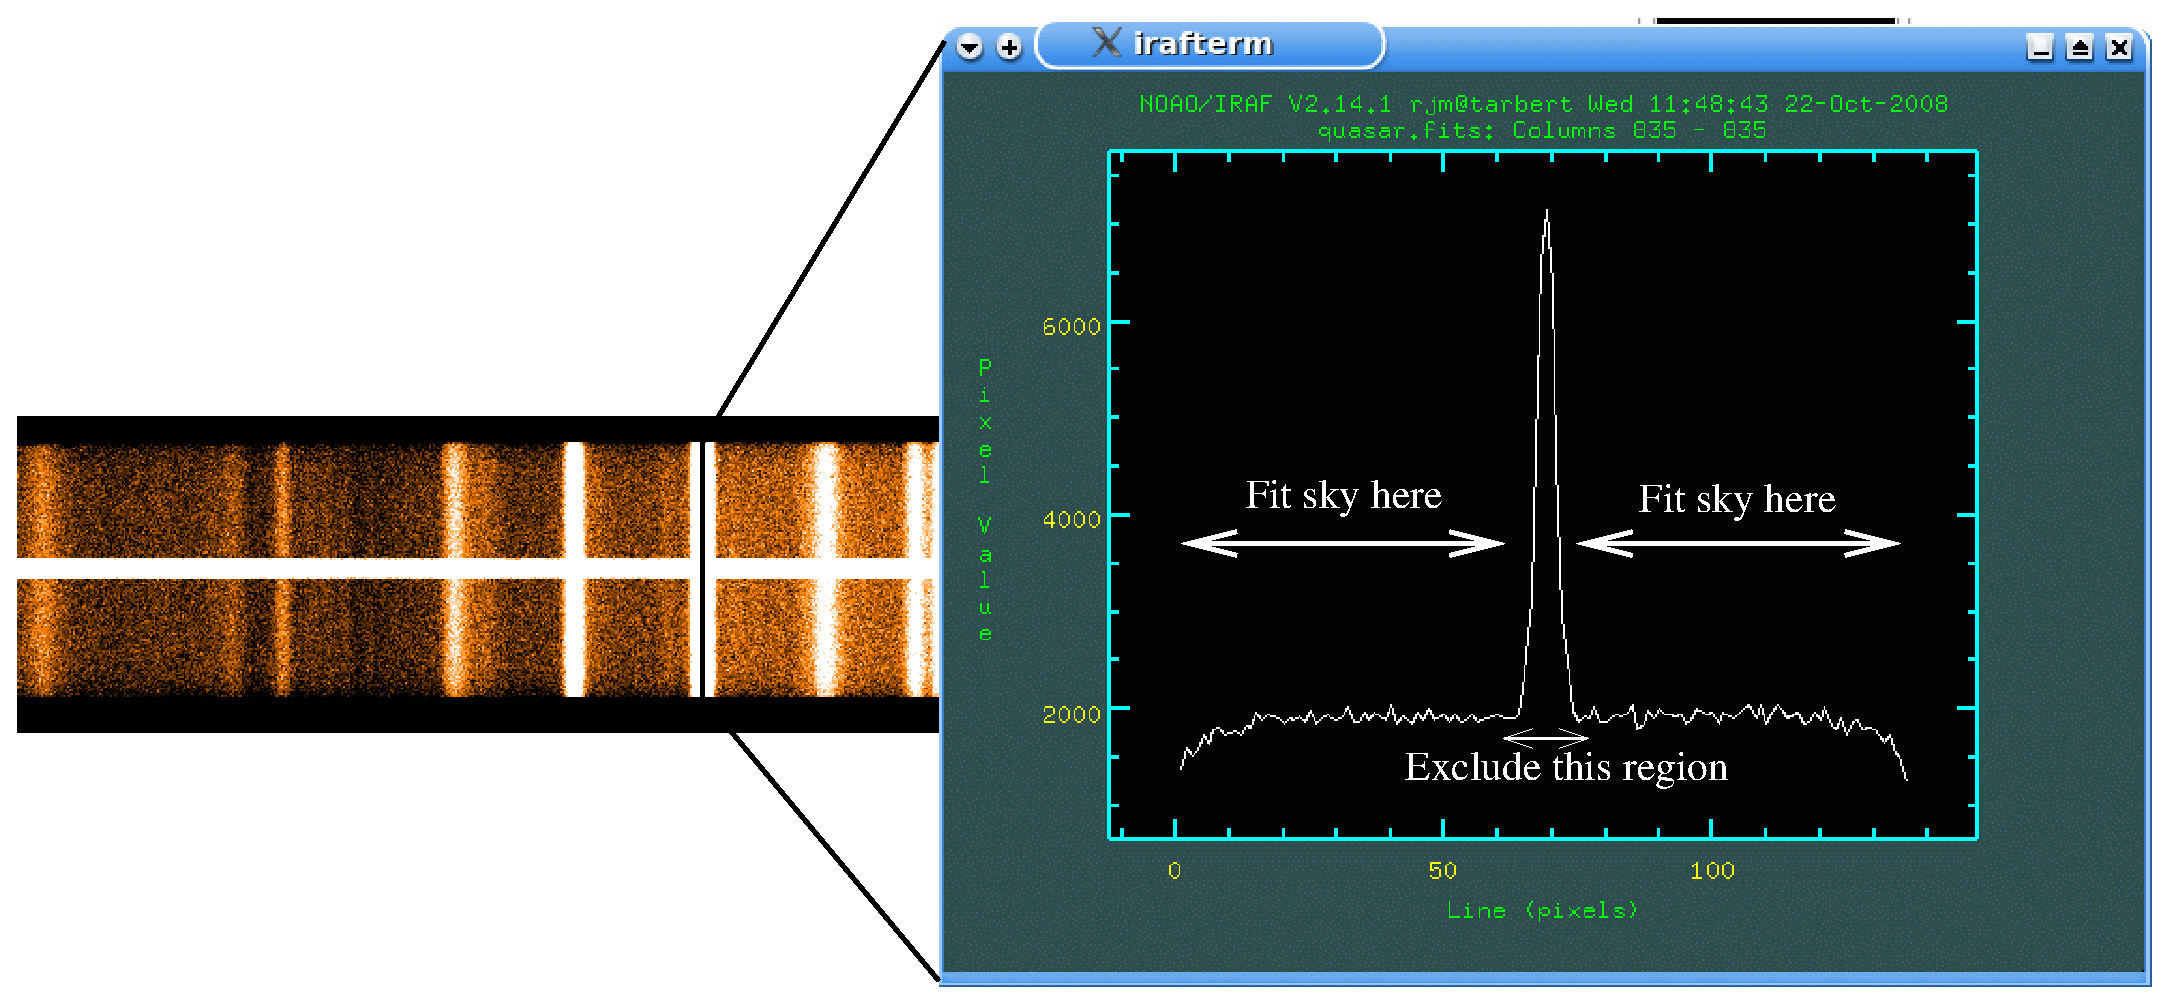
\psfig{file=spectrum_fig2.ps,width=16.0cm,angle=0}}
\caption{Illustration of how the {\sc iraf} task {\it background}
subtracts the sky background from 2D spectra by fitting either side of
the object spectrum.}
\end{figure}

Make sure that you now have a new file in your home directory which is
the flatfielded quasar spectrum with the sky background removed.


{\large {\bf 6. Extracting the quasar spectrum }}

The next stage of the reduction process is to turn the two-dimensional
quasar spectrum into one-dimensional spectrum of flux versus
x-pixel. This process is know as {\it extracting} the spectrum and is
performed with an {\sc iraf} task called {\it apsum}. At the command
prompt, type:

{\tt apsum quasarskysub.fits}

(If you are asked how many apertures to identify, simply type: 1 $<$return$>$.  If you are asked to edit/trace apertures or clobber
the existing output image, type `no', but if asked to extract the aperture spectra or write to database, type `yes'.)

This will produce a file called ``quasarskysub.ms.fits'' which is your
one-dimensional spectrum. To extract the one-dimensional spectrum
{\it apsum} performs the following operation: at each x-pixel
position in the two-dimensional spectrum, {\it apsum} detects which y-pixels
are dominated by the quasar spectrum and simply adds the flux in those pixels
together. The final result of this process is a one-dimensional
spectrum of flux versus x-pixel value. The range of y-pixels dominated
by the quasar spectrum is referred to as the extraction {\it
aperture}, which explains why the task is called {\it apsum}.

At this stage you can take a first look at your one-dimensional quasar
spectrum using the {\sc iraf} task {\it splot} (spectra-plot). At the
command prompt type:

{\tt splot quasarskysub.ms.fits}

As well as simply displaying spectra, the {\it splot} task allows you
to perform many basic analysis tasks (ask the demonstrator to show you
how it works).Note that if you need to close {\it splot} for any reason,
it is imperative that you press ``q'' within the window first. The command
line prompt should then reappear and it is safe to close the {\it splot} window - 
if you do not do this {\sc iraf} will crash and you will have to start over.



{\large {\bf 7. Wavelength calibration}}

\begin{figure}
\centerline{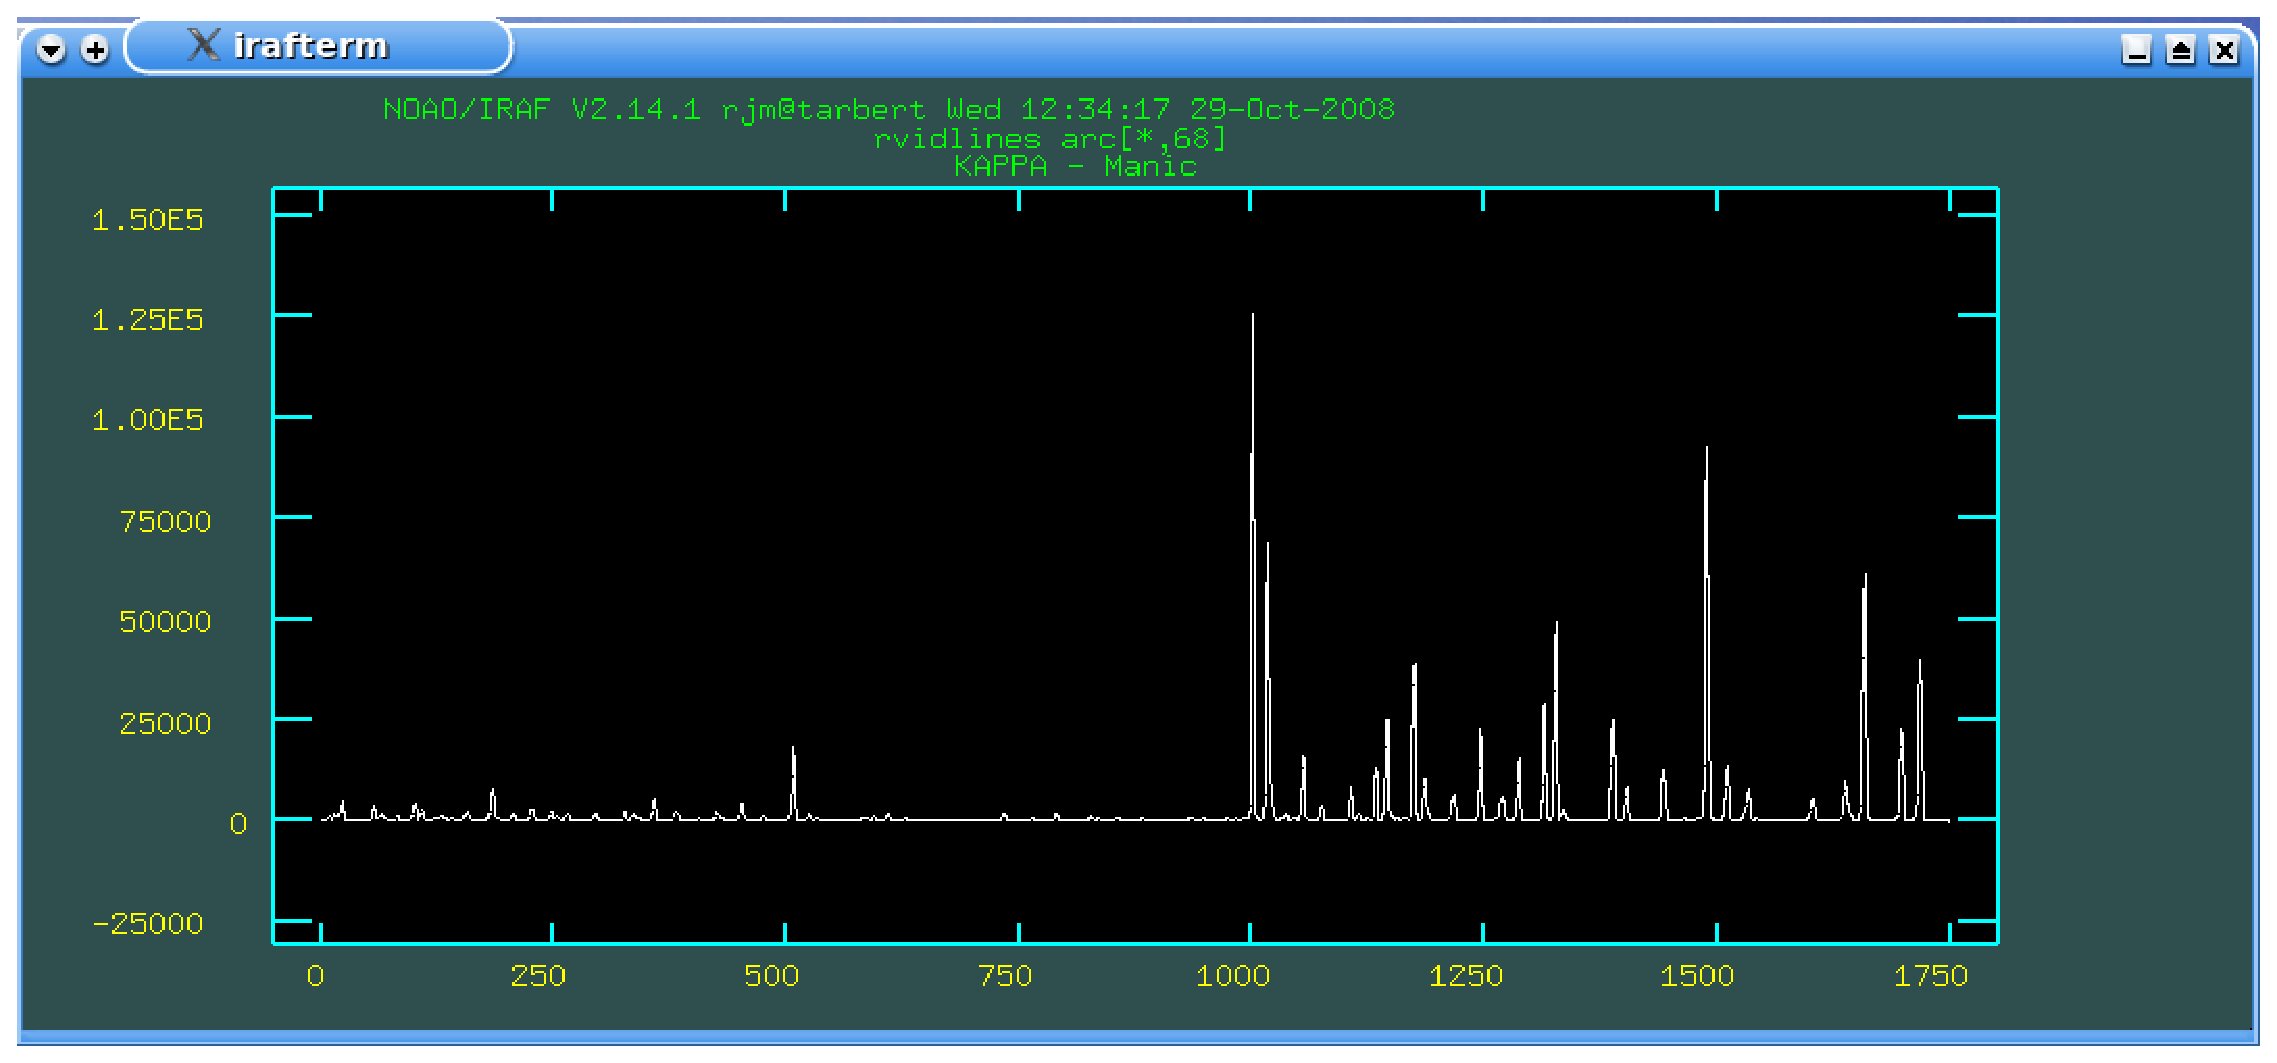
\psfig{file=arc.ps,width=16.0cm,angle=0}}
\caption{{\sc iraf} window generated by {\it identify} showing the
arc spectrum}
\end{figure}

The next stage in the reduction process is to perform the wavelength
calibration. At present, the one-dimensional spectrum of the quasar is
simply flux versus x-pixel number, and we need to
convert this into a one-dimensional spectrum of flux versus
wavelength. To achieve this we have to analyse a so-called ``arc
spectrum'', which is a spectrum of a gas discharge tube containing
elements\footnote{in this case helium, neon and argon} which produce emission lines at known laboratory
wavelengths. By studying the arc spectrum it is therefore possible to
perform the transformation between x-pixels and wavelength. The
wavelength calibration is performed using the {\sc iraf} task {\it
identify}. At the command prompt, type:

{\tt identify arc.fits}

Which should open a new window showing the arc spectrum (see Fig 5). 
In order to make the identification of the arc lines easier, it
may be worthwhile extending the new window horizontally (ask the
demonstrator how to do this).

Now for the tricky bit. You need to compare this arc spectrum with that
contained in the {\em CCD Atlas of Helium/Neon/Argon Spectra} (see Appendix\footnote{note: one of the 
arc lines has the wrong wavelength in the appendix}), 
in order that you can identify $\simeq 20$ lines of known wavelength, preferably
scattered reasonably well through the spectral range. 
It is a good idea to print out your arc spectrum, so that you can write
wavelengths on it for those lines that you believe you have identified.
As a clue, the bright line at pixel number 500 is the 5015.675 \AA\ line
which comes before a region of much weaker emission lines, and the bright
line at pixel number 1000 is the 5852.4878\AA\ line which comes at the red
end of this emission-line ``desert''. 


To identify the lines, click on the {\it identify} window to activate
it, place the cursor over the arc line of interest and press the ``m''
key to mark the line. At this point you will be asked to enter the
wavelength of the arc line. Repeat this process
until you have identified $\simeq20$ arc lines. Once you have
identified enough arc lines you can press ``f'' to fit the dispersion
solution. The {\it identify} window will update to show you the fit,
at which point you can delete outlier points with the ``d'' key and
re-fit the solution by pressing ``f'' once again. Once you are happy
with the quality of the fit (all points within $\simeq1$\AA\,) press
``q'' twice to exit {\it identify}, and then confirm that you want to 
write the dispersion solution to the database.

To let {\sc iraf} know that you want to associate this dispersion
solution with your one-dimensional quasar spectrum, the {\sc iraf} package {\it hedit} (header edit) can be used. To add
the keyword ``REFSPEC1'', type:

{\tt hedit quasarskysub.ms.fits fields=REFSPEC1 value=arc.fits add=yes}

And finally, to apply the wavelength calibration to your quasar
spectrum, type:

{\tt dispcor quasarskysub.ms.fits \verb,quasarskysub_wave.ms.fits,}

The task {\it dispcor} reads the keyword you have just added, pointing to the solution for {\sc arc.fits}, and
applies this to the image.

{\large {\bf 8. Redshift determination}}

You can now view your final wavelength calibrated spectrum by typing:

{\tt splot \verb,quasarskysub_wave.ms.fits,}

Using {\it splot} note down the wavelengths of any obvious emission
lines in the quasar spectrum using the cursor and by pressing the space bar.

\bigskip

Redshift $z$ is defined by the equation

$$\lambda_{observed} = (1 + z) \lambda_{emitted}$$

and so if you can work out which emission lines these actually are, then
it is trivial to calculate the redshift. Moreover, you will know if
you have identified the emission lines correctly because then 
the calculation of redshift from each emission line will give the same
value of $z$ to an accuracy of typically 3 decimal places.

A list of the brightest emission lines seen in active galaxies and
quasars is given below, along with their laboratory wavelengths. 
Only a few of these lines are ever visible in the optical spectrum of a given quasar, and
precisely which ones are visible obviously depends on its actual redshift.
 
By a process of elimination, work out which of these lines are visible in
your reduced spectrum, and hence calculate the redshift of the quasar,
quoting an accuracy based on the line-by-line variation in $z$. {\bf It is important that
you clearly demonstrate in your report how you determined the quasar redshift.}

{\large {\bf 9. Saving plots for your report}}

For the purposes of writing your final report you may want to include
plots of the various stages of the reduction process.

Within {\sc iraf} you can generate
postscript copies of the plots generated by {\it splot, identify} etc
by typing:

{\tt :.snap eps}

in the appropriate window. This will produce a postscript ``.eps''
copy of the {\sc iraf} window in your directory which can be viewed
with ghostview (gv) and then printed.


\begin{center}

{\bf Table: Prominent UV/optical emission lines in quasars}

\begin{tabular}{ll}

Lyman$-\alpha$  \hspace*{2cm} & 1215\AA \\
NV                            & 1240\AA \\
CIV                           & 1549\AA \\
CIII                          & 1909\AA \\
MgII                          & 2799\AA \\
HeI                           & 3189\AA \\ 
$[$ NeV $]$                   & 3426\AA \\
$[$ OII $]$                   & 3728\AA \\
$[$ NeIII $]$                 & 3870\AA \\
$[$ NeIII $]$                 & 3961\AA \\
H-$\delta$                    & 4103\AA \\
H-$\gamma$                    & 4346\AA \\
H-$\beta$                     & 4861\AA \\
$[$ OIII $]$                  & 4959\AA \\
$[$ OIII $]$                  & 5007\AA \\
$[$ OI $]$                    & 6300\AA \\
H-$\alpha$                    & 6563\AA \\
$[$ SII $]$                   & 6724\AA \\

\end{tabular}

\end{center}